\resizebox*{15cm}{!}{
	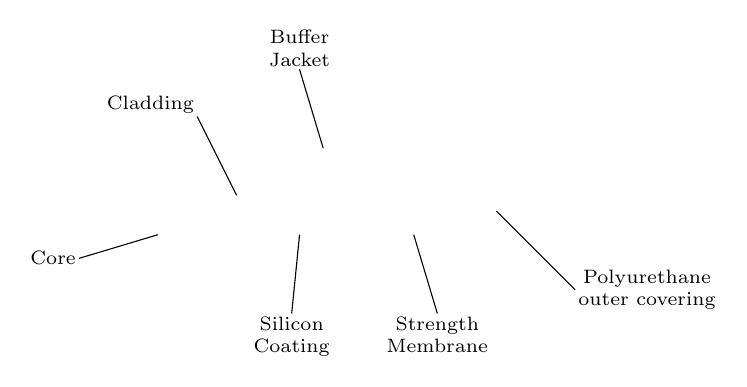
\begin{tikzpicture}[inner sep=1pt, font=\scriptsize]
		\cylinder{.3}{.75}{.7}{1.5}{1}{.2}{blue!25!white}
		\cylinder{-.5}{.55}{.6}{1.5}{.8}{.2}{green!25!white}
		\cylinder{-1.2}{.4}{.5}{1.5}{.7}{.15}{yellow!25!white}
		\cylinder{-1.8}{.25}{.4}{1.5}{.6}{.15}{orange!25!white}
		\cylinder{-2.3}{.15}{.3}{1.5}{.5}{.1}{red!25!white}
		\cylinder{-3}{0}{.1}{1.5}{.65}{.15}{white}
	
		% labels
		\draw (-3, 0) -- ++(-1, -.3) node[anchor=east] {Core};
		\draw (-2, .5) -- ++(-.5, 1) node[anchor=south east] {Cladding};
		\draw (-1.2, 0) -- ++(-.1, -1) node[anchor=north, align=center] {Silicon\\ Coating};
		\draw (-.9, 1.1) -- ++(-.3, 1) node[anchor=south, align=center] {Buffer\\ Jacket};
		\draw (.25, 0) -- ++(.3, -1) node[anchor=north, align=center] {Strength\\ Membrane};
		\draw (1.3, .3) -- ++(1, -1) node[anchor=west, align=center] {Polyurethane\\ outer covering};
	\end{tikzpicture}
}